\documentclass[main.tex]{subfiles}

\begin{document}

  \section{Examples and timings}\label{sec:examples_timings}

    \newcommand{\bern}{\mathcal{B}}
  \newcommand{\bernrev}{\widetilde{\bern}}

  For testing purposes we consider a family of curves given by Bernoulli polynomials
          \begin{equation*}
              \bern_{m,n} : y^m = B_n(x) = \sum_{k=0}^n\binom nkb_{n-k}x^k
          \end{equation*}
  as well as their reciprocals
  \begin{equation*}
  \bernrev_{m,n} : y^m = x^nB_n\left(\frac1x\right).
  \end{equation*}

  The branch points of these curves present interesting patterns which can be respectively considered
  as good and bad cases from a numerical integration perspective (Figure \ref{m-fig:roots_bern}).

  \begin{figure}[H]
      \begin{center}
          \subfloat[$\bern_{m,8}$]{ 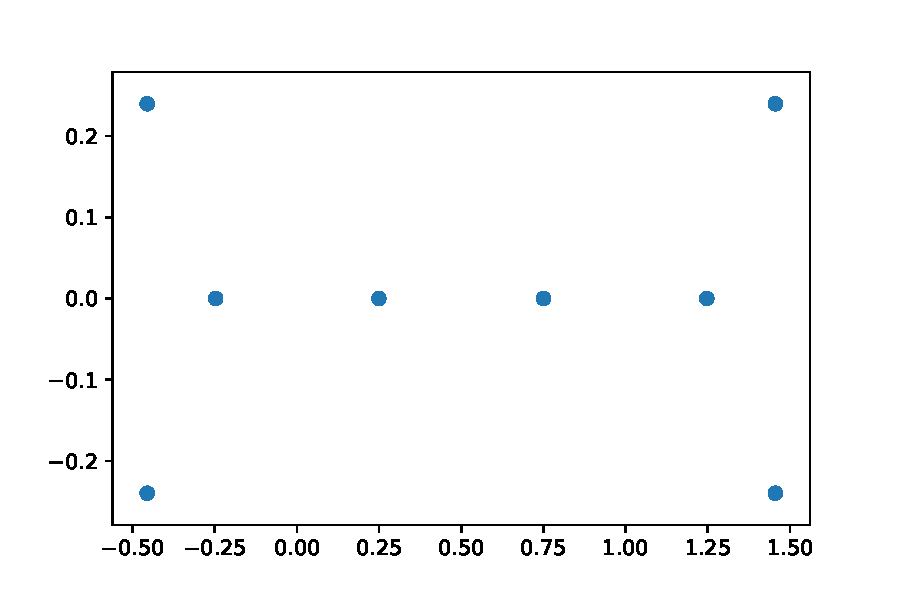
\includegraphics[width=.4\linewidth,page=1]{images/roots_bern.pdf} }
          \subfloat[$\bern_{m,30}$]{ \includegraphics[width=.4\linewidth,page=2]{images/roots_bern.pdf} }\\
          \subfloat[$\bernrev_{m,8}$]{ \includegraphics[width=.4\linewidth,page=3]{images/roots_bern.pdf} }
          \subfloat[$\bernrev_{m,30}$]{ \includegraphics[width=.4\linewidth,page=4]{images/roots_bern.pdf} }
      \end{center}
      \caption{configurations of branch points.}
  \label{fig:roots_bern}
  \end{figure}

  In the case of hyperelliptic curves, we compare our timings with the existing
  Magma code \cite{vanWamelen06} (see Tables \ref{tab:time_hyp} and \ref{tab:time_sup}).
  We obtain a huge speedup which is mostly due
  to the better integration scheme, but more interesting is the fact that the
  running time of our algorithm mainly depends on the genus and the precision,
  while that of Magma depends a lot on the branch points and behaves very badly
  in terms of the precision.

  \begin{table}[H]
      \begin{center}
          \begin{tabular}{lllrrrrr}
              \toprule
              & & \hfill bits & 128 & 512 & 2000 & 4000 & 10000 \\
              genus & curve & \hfill digits & 38 & 154 & 600 & 1200 & 3000 \\
              \midrule
              3 & $\bern_{2,8}$
              &   Arb         & 5e-3  & 0.01  & 0.16    & 0.48     & 3.99 \\
              & & Magma (new) & 0.05  & 0.08  & 0.44   & 2.16    & 25.3 \\
              & & Magma (old) & 0.33  & 0.44  & 6.28   & 421  & --- \\
              \cmidrule{3-8}
              & $\bernrev_{2,8}$
              &   Arb         & 5e-3  & 0.01  & 0.17    & 0.54      & 4.58 \\
              & & Magma (new) & 0.06  & 0.11  & 0.67   & 3.42     & 40.6 \\
              & & Magma (old) & 0.42  & 0.45  & 6.44   & 457   & --- \\
              \midrule
              14 & $\bern_{2,30}$
                & Arb         & 0.05  & 0.22   & 1.99    & 8.74     & 80.9 \\
              & & Magma (new) & 0.55  & 0.94  & 4.64   & 18.7   & 185.1 \\
              & & Magma (old) & 5.15  & 10.1 & 134 & 9291 & --- \\
              \cmidrule{3-8}
              & $\bernrev_{2,30}$
              &   Arb         & 0.05  & 0.23   & 2.11    & 9.31      & 87.8 \\
              & & Magma (new) & 0.51  & 1.02  & 5.40   & 21.9    & 227 \\
              & & Magma (old) & 14.8  & 42.6  & 370 & 12099 & --- \\
              \midrule
              39 & $\bern_{2,80}$
              &   Arb         & 0.69 & 1.64   & 16.1   & 70.5    & 601 \\
              & & Magma (new) & 6.29  & 9.08  & 36.4  & 122  & 1024 \\
              \bottomrule
          \end{tabular}
          \caption{timings for hyperelliptic curves, single core Xeon E5 3GHz (in seconds).}
          \label{tab:time_hyp}
      \end{center}
  \end{table}

  \begin{table}[H]
      \begin{center}
          \begin{tabular}{lllrrrrr}
              \toprule
              & & \hfill bits & 128 & 512 & 2000 & 4000 & 10000 \\
              genus & curve & \hfill digits & 38 & 154 & 600 & 1200 & 3000 \\
              \midrule
              21 & $\bern_{7,8}$
              &   Arb         & 0.06 & 0.27   & 4.25    & 29.5    & 455 \\
              & & Magma (new) & 0.23  & 1.06  & 14.6  & 83.1   & 1035 \\
              \cmidrule{3-8}
              & $\bernrev_{7,8}$
              &   Arb         & 0.03 & 0.19  & 7.44    & 58.8   & 1027 \\
              & & Magma (new) & 0.30  & 1.64  & 23.9  & 132 & 1613 \\
              \midrule
              84 & $\bern_{25,8}$
              &   Arb         & 0.09   & 0.45   & 8.86     & 55.6    & 727 \\
              & & Magma (new) & 0.74   & 2.60   & 27.2   & 135  & 1529 \\
              \midrule
              87 & $\bern_{7,30}$
              &   Arb         & 2.05  & 6.46   & 43.9   & 249   & 3091 \\
              & & Magma (new) & 2.29  & 10.0 & 93.8  & 461  & 4990 \\
              \midrule
              348 & $\bern_{25,30}$
              &   Arb         & 2.82   & 9.57    & 101  & 557   & 6195 \\
              & & Magma (new) & 19.9  & 41.4  & 234  & 1014 & 9614 \\
              %\midrule
              %237 & $\bern_{7,80}$
              %&   Arb         & 45.687 & 123.13 & 369.24  & 1688.10  & 16545.16 \\
              %& & Magma (new) & 22.500 & 69.550 & 594.520 & 2591.710 & 24666.250 \\
              \midrule
              946 & $\bern_{25,80}$
              &   Arb         & 67.8  & 182  & 952   & 4330 \\
              & & Magma (new) & 369 & 585 & 2132 & 7474 \\
              \bottomrule
          \end{tabular}
          \caption{timings for superelliptic curves, single core Xeon E5 3GHz (in seconds).}
          \label{tab:time_sup}
      \end{center}
  \end{table}

  \biblio
  \end{document}
